% define document class and set class options
\documentclass[11pt, a4paper]{article}

%===============================================
% *** LIST OF GENERAL PACKAGES *** %
% language package (french option available as well)
\usepackage[english]{babel}

% input fonts
\usepackage[utf8]{inputenc}
\usepackage[T1]{fontenc}
\usepackage{csquotes}

% customize default page geometry (size of margins, ...)
\usepackage{geometry}
\geometry{hmargin=2cm,vmargin=3cm}
\usepackage{titling}

\usepackage{titlepage}

% writing style
\usepackage{lmodern}
\usepackage{times}	 

% include images (image extensions & paths)
\usepackage{graphicx}
\DeclareGraphicsExtensions{.pdf,.jpg,.png,.eps}
\graphicspath{{figs/}}

\usepackage{wrapfig}

% display hyperlinks in the text
\usepackage{hyperref}  %
\hypersetup{colorlinks,%
            citecolor=red,%
            filecolor=black,%
            linkcolor=blue,%
            urlcolor=blue,%
            breaklinks=true}
            
% customize enumerated lists
\usepackage{enumitem}

% lipsum command to fill in the document (for visualisation purposes)
\usepackage{lipsum}

%===============================================
% *** CAPTIONS AND SUBFIGURES *** %
\usepackage{subcaption}

%===============================================
% *** TABLES *** %
\usepackage{booktabs}
\usepackage{multirow}

%=============================================== 
% *** BIBLIOGRAPHY (FOR BIBLATEX) *** %
\usepackage[
    backend=biber,
    style=ieee,
    ]{biblatex}

\usepackage{bookmark}
\addbibresource{bgtg_lib.bib}

% citation style: apa, ieee, authoryear, ...

%===============================================
% *** MATHS / PHYSICS PACKAGES *** %
\usepackage{amsfonts,amssymb,amsmath,amsthm}
\usepackage{mathrsfs}
\usepackage{mathtools}  % for DeclarePairedDelimiter
\usepackage{siunitx}    % notation physical units

% notations (shortcuts)
\newcommand{\bs}[1]{\boldsymbol{#1}}
\newcommand{\nbpix}{N}
\DeclareMathOperator{\prox}{prox}
\DeclareMathOperator{\sgn}{sgn}
\DeclareMathOperator*{\argmin}{argmin}
\DeclarePairedDelimiter{\norm}{\lVert}{\rVert}

%===============================================
% *** TITLE, AUTHOR AND DATE *** %
\pretitle{\begin{center}\fontsize{30bp}{30bp}\selectfont}
\posttitle{\par\end{center}}

\preauthor{\begin{center}\fontsize{14bp}{14bp}\selectfont}
\postauthor{\par\end{center}}
%===============================================
% *** MAIN DOCUMENT *** %
\begin{document}

% \begin{titlepage}
\centering
% Logos
\begin{minipage}{.25\linewidth}
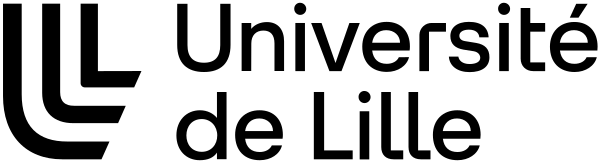
\includegraphics[width=\linewidth]{../images-figures/ulille.png}
\end{minipage}
\hfill
\begin{minipage}{.25\linewidth}
\centering

\includegraphics[width=\linewidth]{../images-figures/Centrale-Lille-Ecole.png}
\end{minipage}
\hfill
\begin{minipage}{.25\linewidth}

\includegraphics[width=\linewidth]{../images-figures/imt.png}
\end{minipage}

\vfill

% Subtitle

{\large Research project final report \\ \textit{March 2025} \vspace{1\baselineskip}}

% Title
\begin{minipage}{\linewidth}
\huge
\bfseries
\centering
\rule{\linewidth}{1.5pt}\\
Conditional Generation of Bass Guitar Tablature for Guitar Accompaniment in Western Popular Music\\[-3mm]
\rule{\linewidth}{1.5pt}
\end{minipage}

\vfill

% Persons involved 
\begin{minipage}{.45\linewidth}
\textit{Student:}\\
Olivier \textsc{Anoufa}\\
\textit{Data Science Master 2}

\end{minipage}
\hfill
\begin{minipage}{.45\linewidth}
\flushright
\textit{Supervisors:}\\
Alexandre \textsc{D'Hooge}\\
Ken \textsc{Déguernel}\\
\textit{Algomus team, CRIStAL}
\end{minipage}

\vfill

% Abstract
\begin{flushleft}
\justify
\textbf{Abstract ---} The field of symbolic music generation has seen great advancements with the rise of transformer-based architectures.
Addressing a specific need identified through a user study conducted on guitar players, we focus on developing AI tools to generate bass guitar tablatures conditioned on scores of other instruments in Western popular music.
The bass guitar, a crucial component of the rhythmic and harmonic sections in music, presents a unique challenge due to its dual role in providing structure and groove.
Building upon the tablature notation, the most popular way to share music among guitarists, this work adopts modern encoding schemes to integrate tablature representation into transformer-based models.
To this end, the project involves preprocessing a large dataset of music scores and fine-tuning state-of-the-art transformer architectures.
Due to the project being the first of its kind and its creative nature, the evaluation of the generated tablatures is mainly done qualitatively.
\vspace{.5\baselineskip}\\
\end{flushleft}
\vfill


% Period
% October 1st --- March 31st
% \vspace{1\baselineskip}\\
\begin{flushleft}
\textbf{Key-words ---} music information retrieval, conditional generation, guitar accompaniment, bass guitar, tablature;
\vspace{.5\baselineskip}\\
% \textbf{Mots-clés \hspace{1ex}---} effets audio, traitement de l'information musicale, traitement du signal différentiable, reproduction sonore, musique assistée par ordinateur.
\end{flushleft}
\vfill

% More logos
\begin{minipage}{.25\linewidth}

\includegraphics[height=3cm]{../images-figures/logoCRIStAL.png}
\end{minipage}
\hspace{7cm}
\begin{minipage}{.25\linewidth}

\includegraphics[height=3cm]{../images-figures/cnrs.png}
\end{minipage}

\end{titlepage}


\begin{figure}[t]% We use titling to put a figure on top of the title page
    \centering
    
\includegraphics[width=.5\linewidth]{logos_empile}
\end{figure}

\title{Automatic detection of orchestral blends from scores}

\author{Olivier \textsc{Anoufa} \\  University of Lille, France \\ Master 1 Data Science: Research project}

{\let\newpage\relax\maketitle}

\newpage

\section*{Introduction}

Many perceptual phenomena are contained in the score, intentionally planned or not by the composer.
A blend is a phenomenon that occurs in orchestral music when several voices fuse together to generate a new timbre\cite{}.
This happens when a listener cannot distinguish the different voices, that is to say the different instruments, that are playing at the same time.
A blend can be intentional or not, the aim of this project is to detect such phenomena in orchestral music scores.

% Blend example from TOGE with legend on part/bar and add references to the figure

However, symbolic music computational analysis is a vast and complex topic that requires a study on the concept of music scores, voices and streams.
To analyse symbolic music, and more precisely to compare parts within a score, we first need to define those terms.

Scores are the written representation of music. They are a way to communicate music to musicians and to listeners.
We will use MusicXML files as scores. MusicXML is a format that allows to represent music scores in a computer-readable format.
Voices in a score is not a concept as simple as it seems. Cambouropolos in 2008 defined three different ways to define voices in a score.
Voices can be simply defined as the sound sequence produced by a single source (an instrument or an individual choral voice).
However, voices can also be defined in a perceptual way, that is to say voices would be delimited by the sound sequences the listeners perceive as distinct.
Finally, voices can be separated based on harmonic theory relative to music composition.
With this definition, voices are delimited by the musical structure of the score\cite{vaswaniAttentionAllYou2023}.

We chose to adopt the term stream, that is an assemble of parts is played by different instruments grouped by perceptual principles.
These definitions are extremely basic but are necessary approximations to be able to extract features for a machine learning model.
Using these definitions, a blend can be defined as a phenomenon that occurs when a stream can not be broken down into parts by a listener.


In this work we focused on concurrent grouping, starting from the lowest level of the taxonomy, classifying blends and non-blends.
This grouping effect arises from the basic technique of combining instruments at the unison or at particular pitch intervals, usually implying rhythmic synchrony and parallelism in pitch.
However, as we will see, not all couplings result in blending of the component instrument.
This first analysis oriented us in our choice of features and machine learning model\cite{}.

Indeed, music can take an infinite number of shapes but an algorithm or machine learning model needs a finite number of inputs\cite{}.
We sorted features into four categories using two questions: is the feature related to a single part or the comparison of two parts?
Is the feature computed on a single bar or is it a global characteristic of the instrument?
All the features were computed on scores taken from the OrchARD dataset\footnote[1]{\url{https://orchard.actor-project.org/about/}}.


Our project is not the first to tackle the problem of identifying blends in orchestral scores, algorithms and experiments have already been developed to detect blends in scores.
The algorithm presented by Aurélien Antoine and al in 2021 used synchronicity, harmonicity and parallelism\cite{}.
However, we think many more features could be decisive for this problem such as timbre characteristics on instruments\cite{}.
Moreover, machine learning models have not been used yet to detect blends in scores while we are convinced it is a promising approach.

Therefore, we decided to build a machine learning model taking as input a score, computing several features and returning a prediction (0/1) for each couple of parts and for each bar of the score.
This model is composed of a classifier (add classifier type when chosen) and a hierarchical clustering algorithm to print out a dendrogram tree of the voices' proximity on each bar.

\newpage

\tableofcontents

\newpage

\section{Data retrieval, feature extraction and feature selection}

As presented before, the data was extracted from the OrchARD dataset.
It is composed of 67 movements' scores written by various composers such as Debussy, Berlioz, Beethoven and many others.
They are accompanied by an annotation table describing every motive - among which blends - that occurs in the score. In total, 2796 blends were annotated.
We have access to the bar where the blend starts and the bar where it ends, the strength of the blend, the instruments involved and other information.
The annotations are such that we could retrieve for each bar and each couple of parts if the pair is blending or not on this bar; these are the labels our model will be trained on.
We didn't take in account the annotated strength of the blends and left it for further studies.

Now that we know what we wanted the model to predict, we needed to extract significant features.
Features are sorted in 4 categories:
\begin{enumerate}
    \item Global Features computed on single parts
    \item Global features computed on couples of parts
    \item Features computed on single parts for each bar
    \item Features computed on couples of parts for each bar
\end{enumerate}

(presentation beamer plan structuré + exemple musique au début récupérer de TOGE voir readme)

\section{Model selection and first iterations}

\section{Model improvement and further iterations}

\section{Conclusion}

ouverture sur le fait que certains facteurs importants ne peuvent pas être pris en compte (attack time, room acoustics, dynamics https://timbreandorchestration.org/writings/timbre-lingo/blend)

\newpage

%\nocite{*} % force display of the full content of the .bib file, w/o any citation in the document
\printbibliography% references: print bibliography (with bibtex file)

\end{document}